\chapter*{Acknowledgments}
\addcontentsline{toc}{chapter}{Acknowledgments}
\novocalize

One of the best things about the Swedish academic environment is its internationality. Not having been exposed to this before starting, it will always remain strong in my mind.

My first and foremost thanks have to go to my two supervisors, Timo Ropinski and Anders Ynnerman, without none of this would have ever happened. TDimo, who would have thought that me applying to a student technician job would ultimately lead to a Diploma thesis, leading to a chance in country, leading to a PhD thesis in Norrk\"oping. I will be ever grateful for the help and the opportunity; I have never looked back and regretted that 24\,h decision to move northwards. Prof.~Ynnerman, thank you for revitalizing my love everything space related and providing the opportunity for me to work on these topics. Anders, tack f\"or att du har introducerat mig f\"or alla intressanta m\"anniskor vid v\aa ra visningar tillsammans. Jag \"ar skyldig dig en drink\footnote{Thank you for all of the interesting people that I met through our shows; I owe you a drink.}!



Thank you to all of my friends and colleagues that I had the pleasure of meeting throughout the years. Indr\.e, thanks for not killing me when someone might have mentioned a historically inaccruate country name; you, Johan and Freja keep fabulous Norrk\"oping safe! Paula, thanks for showing me around in the world and being a good friend and moral compass, you do you! Saghi and Ehsan, \<bAbt mhm tryn t`.tylAt zndgym Az ^smA t^skr myknm>\footnote{Thank you for taking me on the most important vacation of my life}. Daniel, my partner in crime; Umut, [[for being a good friend from the beginning to end and (and afterwards)]]; Erik, for making sure that every paper with your coauthorship gets accepted; Martin, for providing the template and proving to me that it is work to go the extra mile; Stefan, for always being the perfect person to discuss intricacies of algorithmic details with; Khoa, my photography master; Rickard, the Lyapunov (pronounciation) champion; Sathish, shared pain is half the pain; Emil, I really wanted to put a Justin Bieber quote in here, but I couldn't find a fitting one; Joel, whose depth of knowledge about stochastic methods still baffles me; Katerina, Carlo and Lucie, for too many good times to count; Andrew and Sherilyn, to Cologne!; Noeska, bedankt dat je contact met me hebt gehouden, ondanks dat ik gestop ben met MedVis\footnote{Thanks for not breaking off contact even after turning my back on MedVis}; Big thanks also goes, of course, to Joakim, Marcus, \AA sa, Niclas, Jimmy, Andreas, Patric, Miro, Peter, and Jochen. \textgreek{'Euqarist'w 'olouc touc 'Ellhnec f'ilouc mou pou 'ekanan thn p'olh tou} Norrk\"oping \textgreek{endiaf'erousa: El'enh (apo to 'omorfo nhs'i thc K\'uprou), Mar'ia, Nik'olaoc, Apostol'ia, N'ikoc, El'ina kai Bagg'elhc}\footnote{Thanks to all my Greek friends for making the city interesting: Eleni (close enough), Maria, Nikolaos, Apostolia, Nikos, Elina, and Vangelis}.\\ \<hm^cnyn Az tmAm dUstAn AyrAnym `ly, hdyh, ngAr, 'Ar^s, fhymh w mynA t^skr myknm>\footnote{And, of course a big thanks to all my Iranian friends aswell: Ali, Hedieh, Negar, Arash, Fahimeh, and Mina.}

A big thanks to all of the students that I had to pleasure of supervising over the years. You rock! Sandra, Martin, Victor, HC, Jonas, Michal, Anton, Karl-Johan, Tomas, Erik, Kalle, Michael, and Sebastian.

Big thanks to Carter who in many ways is the extact opposite of me, which makes the combination unstoppable; to Masha, thank you for taking me in and for the trust throughout the years of collaboration; to Cl\'audio, for opening up the opportunity for a new exciting life phase.

Vielen Dank auch an meine Familie f\"ur die lebenslange Unterst\"utzung\footnote{Thanks also to my family for the lifetime support}!

And last, but definitely not least, to my incredibly understanding wife Mina. Meeting and marrying someone in the second half of a PhD must be the worst possible time and, yet, she did not run away. I do not have more to say than this: \<`A^sqtm>

\begin{figure}[hb]
\centering
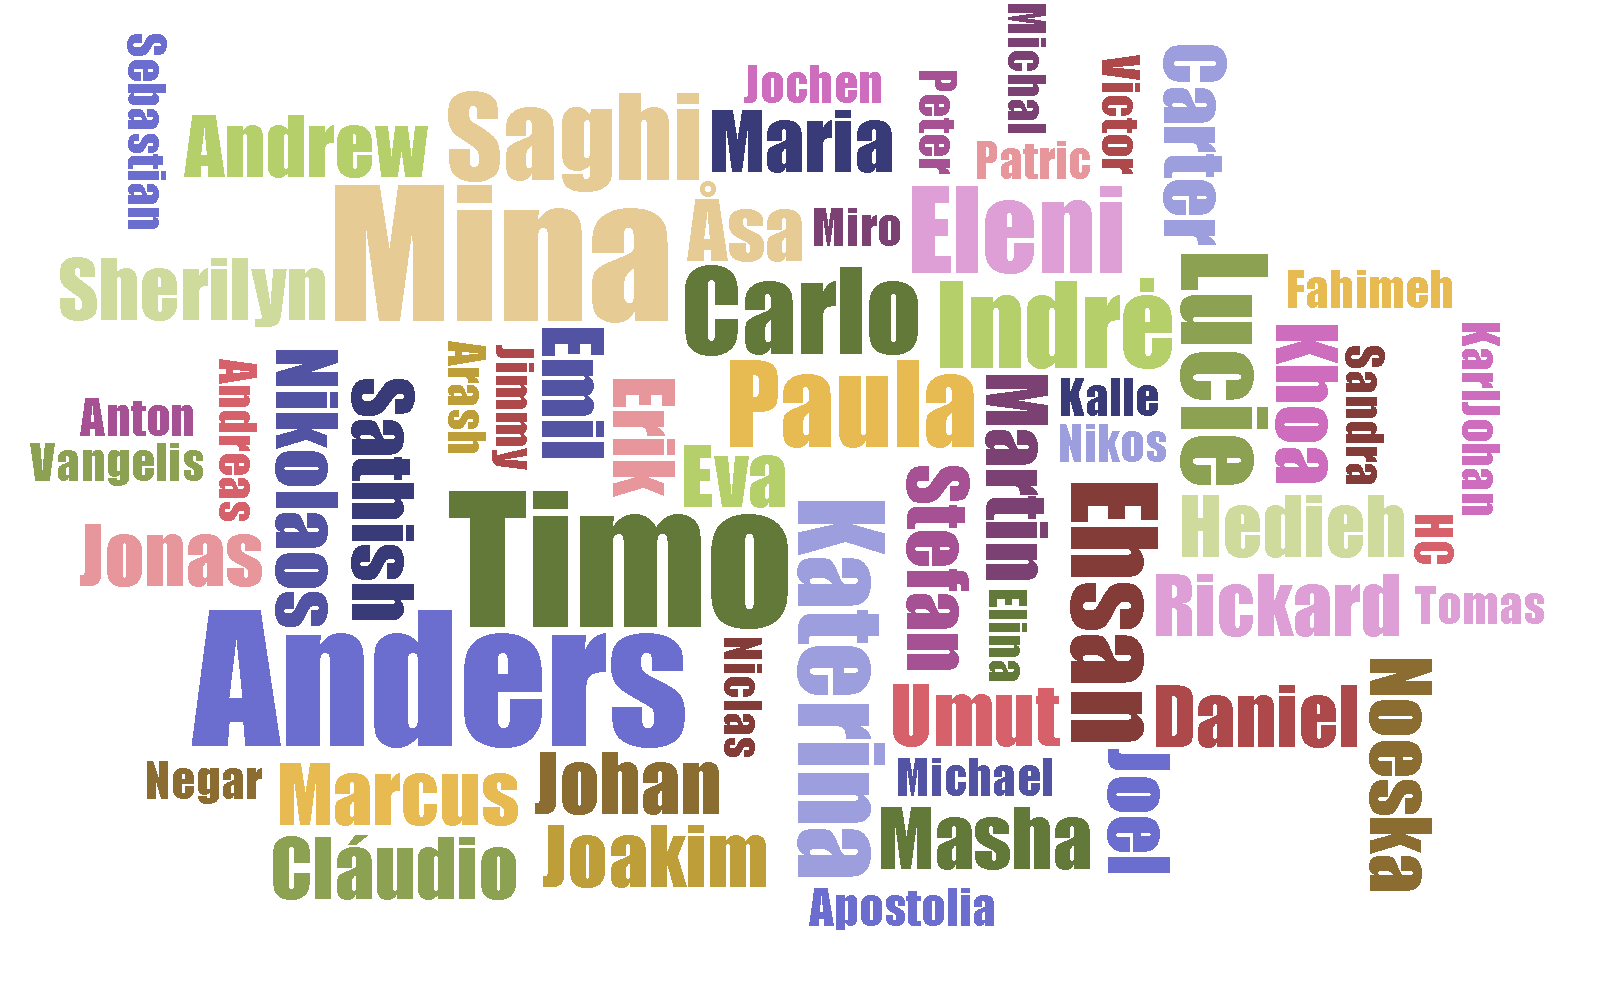
\includegraphics[width=\linewidth]{figures/misc/wordcloud.pdf}
\end{figure}

% Wordcloud source:
% Anders Anders Anders Anders Anders Anders
% Timo Timo Timo Timo Timo Timo
% Mina Mina Mina Mina Mina Mina
% Eva Eva Eva
% Indrė Indrė Indrė Indrė
% Johan Johan Johan
% Paula Paula Paula Paula
% Saghi Saghi Saghi Saghi
% Ehsan Ehsan Ehsan Ehsan
% Daniel Daniel Daniel
% Umut Umut Umut
% Erik Erik Erik
% Martin Martin Martin
% Stefan Stefan Stefan
% Khoa Khoa Khoa
% Rickard Rickard Rickard
% Sathish Sathish Sathish
% Emil Emil Emil
% Joel Joel Joel
% Katerina Katerina Katerina Katerina
% Carlo Carlo Carlo Carlo
% Lucie Lucie Lucie Lucie
% Andrew Andrew Andrew
% Sherilyn Sherilyn Sherilyn
% Noeska Noeska Noeska
% Joakim Joakim Joakim
% Marcus Marcus Marcus
% Åsa Åsa Åsa
% Niclas Niclas
% Jimmy Jimmy
% Andreas Andreas
% Patric Patric
% Miro Miro
% Peter Peter
% Jochen Jochen
% Eleni Eleni Eleni Eleni
% Maria Maria Maria
% Nikolaos Nikolaos Nikolaos
% Apostolia Apostolia
% Nikos Nikos
% Elina Elina
% Vangelis Vangelis
% Hedieh Hedieh Hedieh
% Negar Negar
% Arash Arash
% Fahimeh Fahimeh
% Sandra Sandra
% Victor Victor
% HC HC
% Jonas Jonas Jonas
% Michal Michal
% Anton Anton
% Karl-Johan Karl-Johan
% Tomas Tomas
% Kalle Kalle
% Michael Michael
% Sebastian Sebastian
% Carter Carter Carter
% Masha Masha Masha
% Cláudio Cláudio Cláudio 
\vfill
\hline
\hline

Norrk\"oping, November 2016 \hfill Alexander Bock
\vspace{2cm}
